\subsection{Structures (\textit{CE})}
\subsubsection{Material Selection (\textit{CE})}
\label{section: strcuture material}
Modern-age aircraft exhibit many different structure layouts and material selection for each structure of the aircraft. The goal for the material selection for each section of the aircraft is to meet the given requirements, as well as provide an aircraft which will have the best mechanical performance for the given flight missions. The different structure types evaluated are tabulated in Table \ref{tab:structure_material_table}.

\begin{table}[!h]
\centering
\caption{Structures Build-up Descriptions }
\label{tab:structure_material_table}
\begin{tabular}{ |p{2cm}||p{13cm}| }
\toprule
\multicolumn{1}{|c||}{\textbf{Build-up Type}} & \multicolumn{1}{c|}{\textbf{Description}}                                                                                                                       \\ \hline\hline
Metal                                       & Most or all parts of the primary and secondary structure are metallic, such as aluminum, steel, and titanium alloys                                             \\ \hline
Composite                                    & Most or all parts of the primary and secondary structure are composite, such as carbon fiber reinforced polymers (CFRP), fiberglass, or other composites \\ \hline
Hybrid                                       & Depending on the structure, the material of the structure is either metal or composite                                                                            \\ \bottomrule
\end{tabular}
\end{table}
% \begin{tabular}{ |p{3cm}||p{3cm}|p{3cm}|p{1.5cm}|p{3cm}| }

A metallic build-up is the more traditional method of designing aircraft structures, where most or all primary structures are composed of metal alloys like aluminum, steel, and titanium. This method of construction is typically cost-effective and weight efficient for most structures, however, there are downsides such as damage tolerance and fatigue. A composite build-up requires relatively high development and manufacturing costs using modern technology, but can offer incredible weight-savings and operational cost savings compared to metal structure due to their high strength-to-weight ratio and fatigue and damage tolerance resistance. 

A hybrid build-up is a method where both metals and composites are used for different structures depending on key factors such as fatigue, damage tolerance, ultimate strength per density ratio, cost of manufacturing, assembly methods, and operational costs. Hybrid designs usually reduce overall costs and empty weight of the structure, which results in the wings and stabilizers to be a mainly composite build-up and the fuselage and other secondary structures to be a metal build-up. Hybrid construction is a newer technology, and as the development of manufacturing of composites advances, this style of construction may become more prevalent in industry. A notable aircraft which uses a hybrid build would be the Boeing 777X, in which the wings and stabilizers are composite and the fuselage is metallic. The reason the fuselage is metallic and not composite comes down to the difficulties in manufacturing a round and continuous composite structure, such as the fuselage and empennage sections. A notable aircraft which utilizes mainly composite construction, however, is the Boeing 787. The B787 encountered enormous program overruns in costs and time, mainly stemming from the fuselage construction.

In Table \ref{tab:pugh_structures}, the benefits and costs for each build-up construction method were weighed in a Pugh matrix given the requirements such as cost, manufacturing, and mechanical properties. Cost was weighted the highest due to the RFP requirement which states the proposed aircraft must reduce costs \cite{RFP}.

\begin{table}[!h]
\centering
\caption{Pugh Matrix for Structures Material Selection}
\begin{tabular}{|p{3.5cm}||p{2cm}|p{2cm}|p{2cm}|p{2cm}| }
\toprule
\multicolumn{1}{|c||}{\textbf{Criteria}} & \multicolumn{1}{c|}{\textbf{Weight}} &  
\multicolumn{1}{c|}{\textbf{Metallic}} & \multicolumn{1}{c|}{\textbf{Composite}} & \multicolumn{1}{c|}{\textbf{Hybrid}} \\ \hline \hline 
Cost & 10 & 9 & 7 & 8 \\ \hline
Manufacturability & 8 & 8 & 5 & 7 \\  \hline
Strength to Weight & 8 & 7 & 8 & 9 \\  \hline
Fatigue Rating & 5 & 6 & 8 & 7 \\  \hline
Damage Tolerance & 5 & 7 & 6 & 7 \\  \hline
Corrosion Resistance & 4 & 4 & 9 & 8 \\  \hline
Environmental Impact & 3 & 8 & 4 & 6 \\  \hline \hline
 & \textbf{Total} & \textbf{315} & \textbf{292} & \textbf{328} \\
\bottomrule
\end{tabular}
\label{tab:pugh_structures}
\end{table}
\FloatBarrier

Given the qualitative Pugh matrix, a hybrid construction is most ideal for the given aircraft requirements. This would entail the wingbox and fuselage, including the longerons, frames, and floor joists being constructed from an aluminum alloy. The landing gear will be constructed primary from steel and titanium alloys. The wings and stabilizers, including the skins, ribs, ribs, and stringers would then be modelled using a uni-directional composite material, which assumes isotropic material properties. In reality, composites are anisotropic, but analysis of a directional layup composite is very difficult and not in the scope of this preliminary design. 

In Table \ref{tab:material_selection}, the material composition of each structure can be seen. It can be noticed that all primary structure uses carbon fiber reinforced polymer (CFRP) and epoxy, fiberglass and epoxy, aluminum, steel, or titanium alloys.

% Method 1
\begin{table}[!h]
\centering
\caption{Primary Structure Material Composition}
\begin{tabular}{|p{3.5cm}||p{2cm}|p{6cm}| }
\toprule
\multicolumn{1}{|c||}{\textbf{Structure}} & \multicolumn{1}{c|}{\textbf{Components}} & \multicolumn{1}{c|}{\textbf{Material}} \\ \hline \hline 
\multirow{4}{*}{Wing} & Skin & \multirow{4}{*}{CFRP/Epoxy} \\
                     & Ribs & \\
                     & Spars & \\
                     & Stringers & \\ \hline
\multirow{4}{*}{Horizontal Stabilizer} & Skin & \multirow{4}{*}{CFRP/Epoxy or Fiberglass/Epoxy} \\
                     & Ribs & \\
                     & Spars & \\
                     & Stringers & \\ \hline
\multirow{4}{*}{Vertical Stabilizer} & Skin & \multirow{4}{*}{CFRP/Epoxy or Fiberglass/Epoxy} \\
                     & Ribs & \\
                     & Spars & \\
                     & Stringers & \\ \hline
\multirow{4}{*}{Fuselage} & Skin & \multirow{4}{*}{2024-T4 Aluminum} \\
                     & Longerons & \\
                     & Frames & \\
                     & Wingbox & \\ \hline
\multirow{3}{*}{Landing Gear} & Struts & \multirow{3}{*}{Aluminum, Steel, or Titanium Alloys} \\
                     & Axles & \\
                     & Bulkheads & \\ 
\bottomrule
\end{tabular}
\label{tab:material_selection}
\end{table}
\FloatBarrier

% % Method 2
% \begin{table}[!h]
% \centering
% \caption{Primary Structure Material Composition}
% \begin{tabular}{|p{3.5cm}||p{2cm}|p{6cm}|}\toprule
% \textbf{Structure} & \textbf{Components} & \textbf{Material} \\ \hline \hline 

%     Wing & Skins \newline Ribs \newline Spars \newline Stringers & CFRP/Epoxy \\ \hline
%     Horizontal Stabilizer & Skins \newline Ribs \newline Spars \newline Stringers & CFRP/Epoxy or Fiberglass/Epoxy \\\hline
%     Vertical Stabilizer & Skins \newline Ribs \newline Spars \newline Stringers & CFRP/Epoxy or Fiberglass/Epoxy \\\hline
%     Fuselage & Skins \newline Longerons \newline Frames \newline Wingbox & 2024-T4 Aluminium \\\hline
%     Landing Gear & Struts \newline Axles \newline Bulkheads & Aluminium, Steel, or Titanium Alloys \\ \bottomrule

% \end{tabular}
% \label{tab:material_selection}
% \end{table}

For analysis, the CFRP material chosen was Hexcel AS4C Uni-Directional 3000 filament carbon fiber composite material \cite{hexcel}. In Table \ref{tab:material_properties}, the mechanical properties of 2024-T4 aluminum and CFRP materials being used on the aircraft are tabulated \cite{aluminum}.

\begin{table}[!h]
\centering
\caption{Mechanical Properties of Materials}
\begin{tabular}{|p{3cm}||p{2cm}|p{2.5cm}|p{2.5cm}|p{2cm}| }
\toprule
\multicolumn{1}{|c||}{\textbf{Material Name}} & \multicolumn{1}{c|}{\textbf{Alloy}} &  
\multicolumn{1}{c|}{\textbf{Yield Tensile}} & \multicolumn{1}{c|}{\textbf{Ultimate Tensile}} & \multicolumn{1}{c|}{\textbf{Density}} \\ 
\multicolumn{1}{|c||}{\textbf{}} & \multicolumn{1}{c|}{} &  
\multicolumn{1}{c|}{\textbf{Strength (ksi)}} & \multicolumn{1}{c|}{\textbf{Strength (ksi)}} & \multicolumn{1}{c|}{\textbf{(lb/in$^3$)}} \\ \hline \hline
Aluminum & 2024-T4 & 47 & 68 & 0.1 \\ \hline
Hexcel Carbon Fiber & ASD4 3000 & N/A & 700 & 0.0647 \\
\bottomrule
\end{tabular}
\label{tab:material_properties}
\end{table}


\subsubsection{Construction and Layout (\textit{CE})}
Given the hybrid construction method, the wings and stabilizers require a newer method of construction compared to the traditional metallic construction. Since composite parts are created via a fiber and matrix composition, the stringers can be integrated into the upper and lower panels of the wings and stabilizers via adhesion. This alone saves incredible costs and weight by eliminating the use of fasteners in high-load locations. The absence of fasteners increases the damage tolerance and fatigue rating of the structure as well.

Spars are the most important structure to the wings, and arguably the most important on the entire aircraft. These few parts make the entire aircraft fly, and in the process, see a lot of loading cycles over the life of the aircraft. In metal structures, loading cycles cause fatiguing, and then fatigue cracking, which degrades the structure. Traditionally, metallic structures use a three-piece build-up for the spar: chord on the top and bottom, and a web connecting the two chords. This structure ends-up looking like a C-channel extrusion. The reason the spars are a three-piece build-up comes down to crack growth and fatigue. A crack starts in the lower chord, but cannot grow through the entire spar since the chord is connected to the web by fasteners. There are a few aircraft that have used a one-piece, or monolithic, metallic spar, some being the Boeing 1-B and the Airbus 320 NEO. There is significant research in learning crack-growth patterns and predicting where cracks will start and grow; opening-up huge possibilities in reducing manufacturing costs by allowing optimized metallic spars to be utilized on low-cost aircraft.

The spars are where composites differ greatly from traditional three-piece spar construction. Since composite structures do not crack like metal structures when fatigued, a monolithic spar can be utilized. This spar construction reduces costs, but increases the weight due to a thicker layup compared to a simpler three-piece construction. Due to the considerable cost savings, a monolithic composite spar was modelled, seen in Figs. \ref{fig:spar_layout} and \ref{fig:spar_layout_tip}.

\begin{figure}[!h]
    \centering
    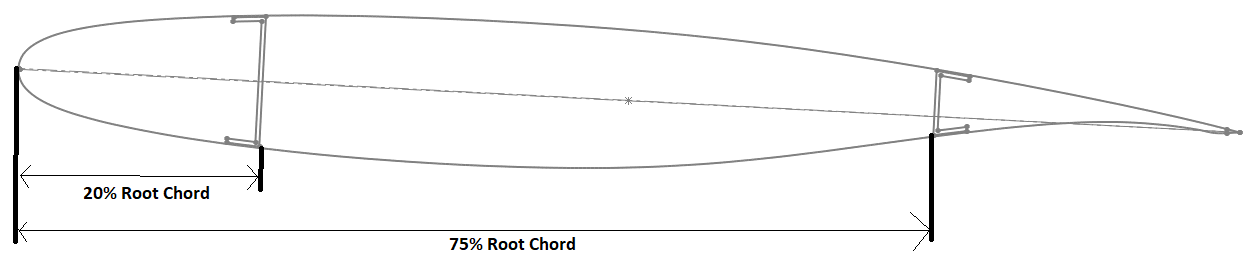
\includegraphics[width=\linewidth]{Photos/structuresandloads/Spar Layout.PNG}
    \caption{SAM Mk I Spar Cross Section at the Wing Root}
    \label{fig:spar_layout}
\end{figure}
\begin{figure}[!h]
    \centering
    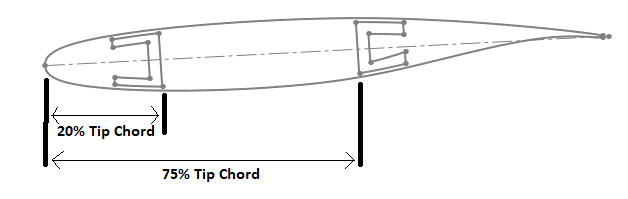
\includegraphics[width=10cm]{Photos/structuresandloads/Spar Layout Tip.PNG}
    \caption{SAM Mk I Spar Cross Section at the Wing Tip}
    \label{fig:spar_layout_tip}
\end{figure}

Ribs in the wings are traditionally multi-piece substructures comprised of machined aluminum parts. The benefit to using aluminum ribs in the wing comes from the fact that composites are difficult to utilize on very complex and dramatic geometry. However, due to manufacturing costs, a multi-piece composite rib was chosen over a monolithic aluminum rib. In an effort to save more cost and manufacturing troubles, a monolithic rib structure, with the rib posts, chords, webs, and pads formed in a single composite part, can be investigated at a later date. Ribs in the stabilizers are typically not as complex as a rib in the wings due to the lower-loaded and smaller structure. In the stabilizers, composite ribs may be utilized for weight savings. The current rib spacing on the wing is 30 inches, which is a derivative of the approximation given by Raymer with a slight adjustment for composite composition \cite{raymer}. This spacing results in 34 ribs in each wing. 

Since the fuselage is a metallic structure, a common layout of frames, stringers, and floor joists can be utilized. The floor joists may be a composite part, as the joists are not primary structure, and the connection method to the frames of the fuselage is by brackets and fasteners. Frames in the business class are spaced with the same distance of the business class seat pitch of 36 inches, and the economy frames are spaced the same distance of the economy seat pitch of 32 inches. The seat pitches are defined in Section \ref{section: internal config}. The frames and longerons are spaced such that no windows or exit doors are covered or physically blocked, where W-shaped longerons are spaced at 10 inches intervals along the fuselage circumference. Several frames will be considered "floating", or not connected to the skin of the fuselage, and others being traditional frames. The floating frames are only mounted to the longerons, rather than the actual skin of the fuselage. Floating frames increase fatigue life, as fewer holes are introduced into the fuselage skin. It will also need to be noted that full frames cannot be present where emergency exit doors and windows exist.

In Fig. \ref{fig:structure_cutaway}, the aircraft structure can be seen. It should be noticed that no windows or doors are covered by frames or stringers in the fuselage. Also note that at this time, the nose ribs have not been modelled, as their current spacing and size is not fully defined for the purposes of this proposal.

\begin{figure}[!h]
    \centering
    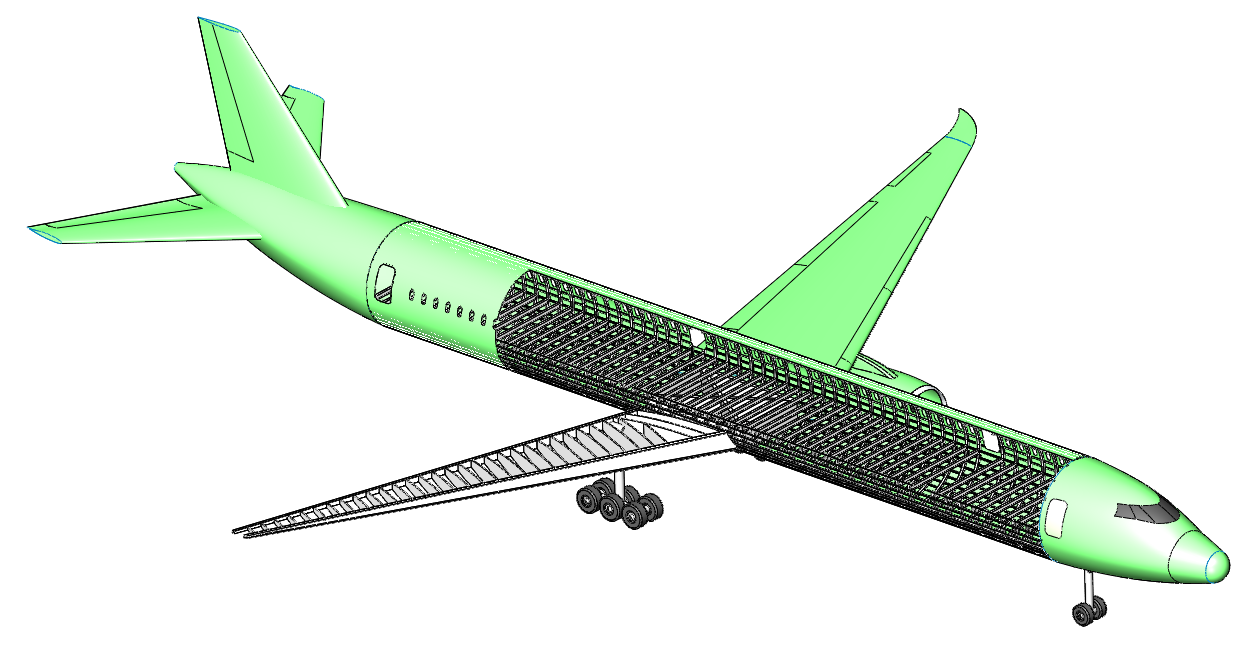
\includegraphics[width=\linewidth]{Photos/structuresandloads/Updated Structures Cutaway.PNG}
    \caption{SAM Mk I Structures Model Cutaway}
    \label{fig:structure_cutaway}
\end{figure}

\subsubsection{Wing Attachment and Configuration}
There are two primary methods of mating the wings and the fuselage: "bolt-on" and "drop-in". These methods are both commonly used in industry, as both offer different advantages and carry their own disadvantages. 

A "bolt-on" method essentially bolts the wings onto the fuselage through the wingbox, as the wingbox is integrated into the fuselage. Utilizing shear plates or tension bolts, each wing is attached to the fuselage using fasteners. This method is preferred by most aircraft manufactures, as manufacturing of the fuselage with an integral wingbox and two separate wings is easier to manage in an assembly line in most cases. Using fasteners to attach the wing to the fuselage from the outside poses a difficult engineering challenge which is to make sure load paths are correctly transferring load to the correct primary structures.

The "drop-in" method refers to dropping the fuselage into the space made by the wingbox and wing superstructure. In this method, the wings and wingbox are a singular structure, and the fuselage does not have an integral wingbox. Due to the wings and wingbox being connected before the mating to the fuselage, a more robust connection to the wingbox (internal connection of the spars to the wingbox, rather than fasteners) can be achieved. 
Given that the aircraft is a wide-body, large wingspan structure, a bolt-on method would be preferred, as the manufacturing and logistical challenges in a "drop-in" method are costly. Choosing to use the bolt-on method, the wing was then designed accordingly. In Fig. \ref{fig:wing_structure}, the wing and wingbox structure can be seen.

\begin{figure}[!h]
    \centering
    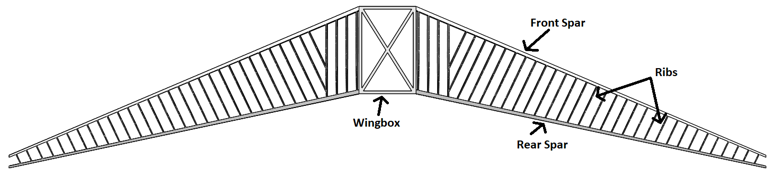
\includegraphics[width=\linewidth]{Photos/structuresandloads/Wing Structure.PNG}
    \caption{SAM Mk I Wing Structure Top View}
    \label{fig:wing_structure}
\end{figure}
\FloatBarrier

It can also be seen in Fig. \ref{fig:wing_structure} that the first 3 inboard ribs of the wing are parallel to the stream-wise direction, with the rest of the outboard ribs being perpendicular to the front spar. This is done to simplify assembly and strength at the root of the wing where the wing attaches to the wingbox. If all of the ribs were perpendicular to the front spar, the first inboard ribs would terminate along the wingbox, complicating the structure.
\clearpage

\subsection{Loads (\textit{MK})}
\subsubsection{V-N Diagram}
\label{subvn}
One important aspect in the structural analysis of the aircraft is determining the limits in the performance of the aircraft. This is done using a V-N diagram, as shown in Figure \ref{figVN}. This diagram incorporates parameters such as wing loading and performance velocities (maneuvering, cruise, and dive velocities) along with limit loading factors. Maximum positive and negative limit loading factors of 2.50 and -1.0 were chosen, respectively, according to the regulations set forth in FAA 14 CFR Part \S 25.337 \cite{cfr}, Limit Maneuvering Load Factors. Additionally, gust loads were added according to FAA CFR Part \S 25.341 \cite{cfr}. The gust load lines were further calculated using a safety factor of 1.5, as specified in FAA 14 CFR Part \S 25.303, Factor of Safety \cite{cfr}. Note that the velocities displayed in the diagram (Figure \ref{figVN}) units displayed as equivalent velocities (KEAS). This V-N diagram was created assuming sea-level conditions. 

\begin{figure}[H]
    \centering
    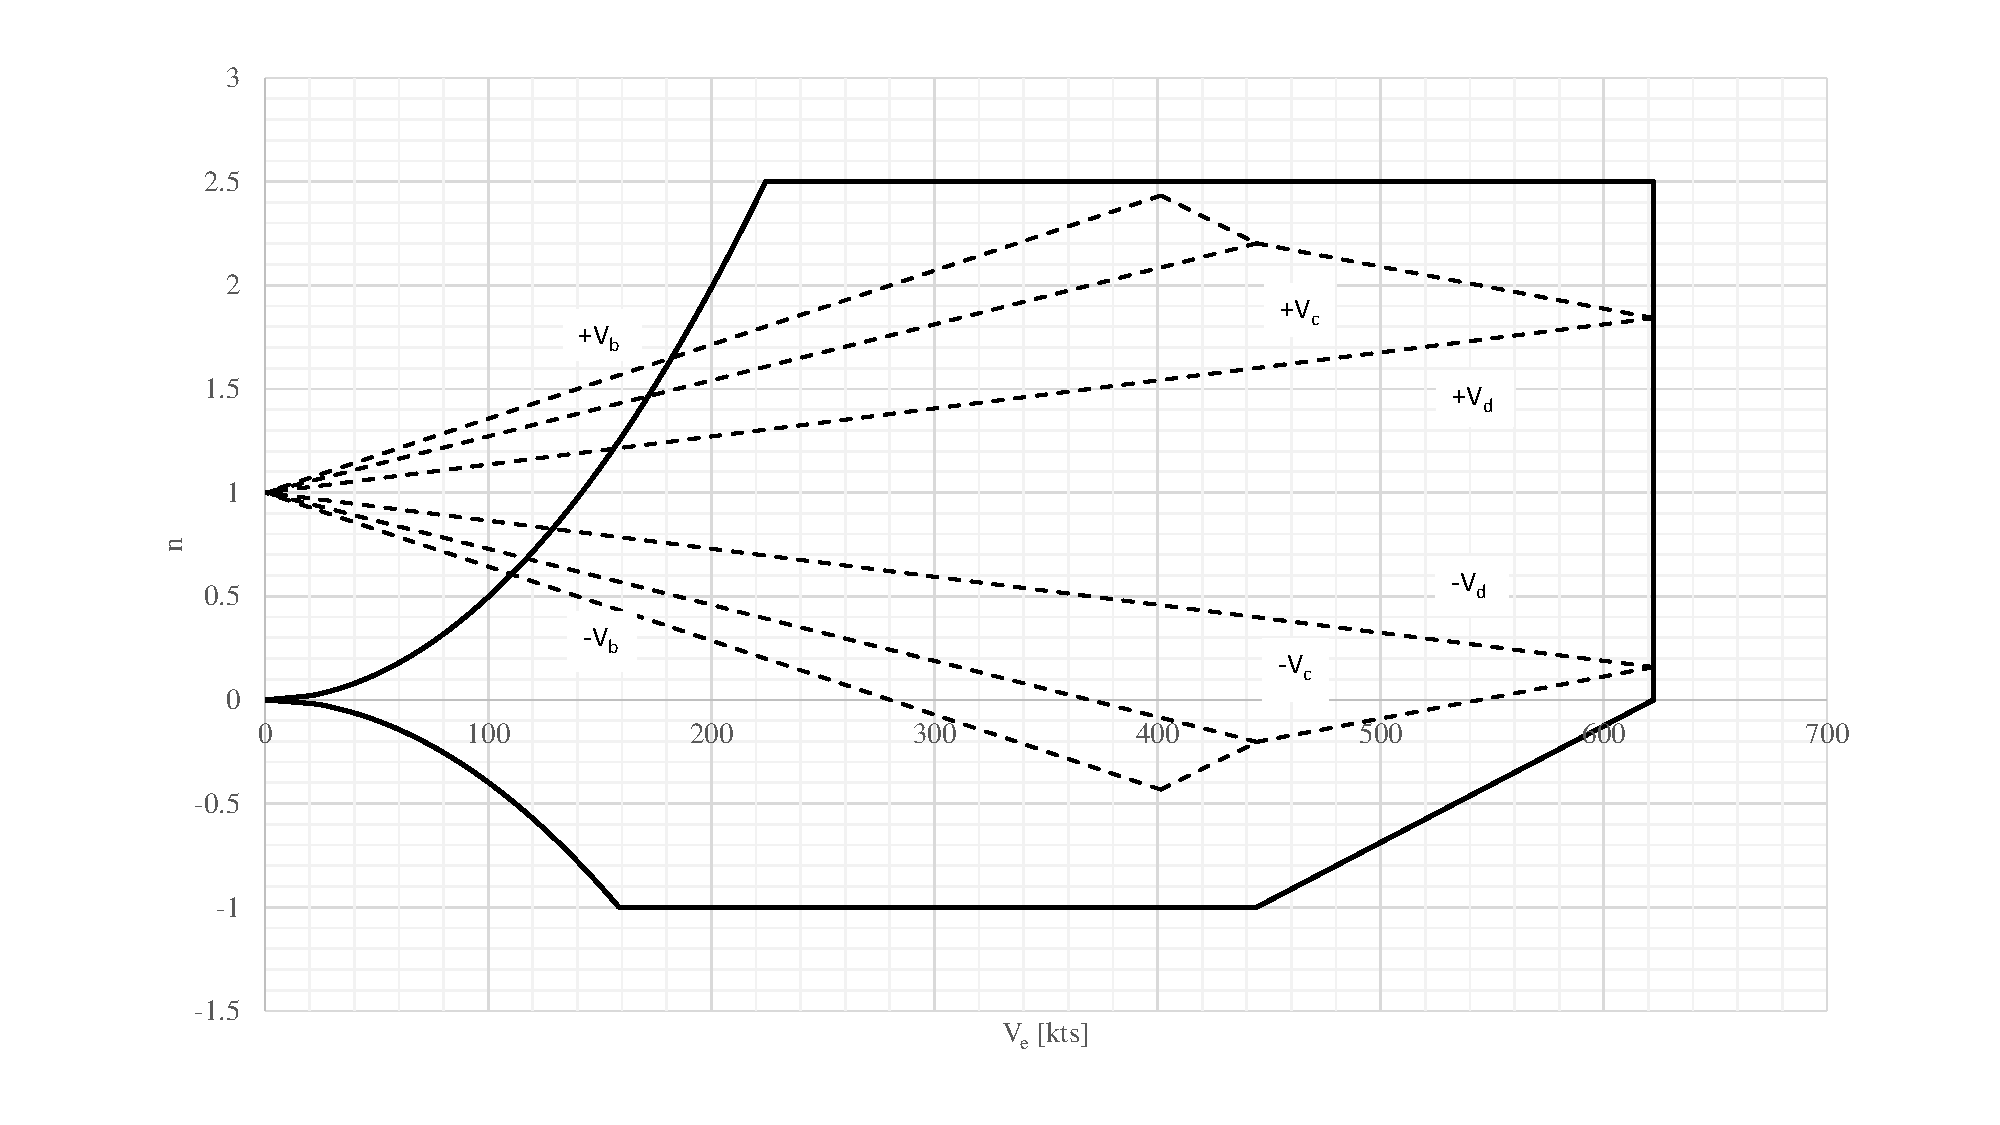
\includegraphics[width=\linewidth]{Photos/VN_Diagram.pdf}
    \caption{V-N Diagram of Limit Load Factors}
    \label{figVN}
\end{figure}

As seen from Figure \ref{figVN}, gust loads do not limit the performance of the SAM Mk I. Moreover, using equations from Roskam \cite{roskam_5}, design maneuvering speed ($V_{A}$), cruising speed ($V_{C}$) and design diving speed ($V_{D}$) were estimated to be 220 kts, 440 kts, and 620 kts, respectively. Furthermore, the calculation of the positive and negative stall lines involved the use of equations from Roskam \cite{roskam_5}. At sea-level and at a limit loading factor of 1 and -1, the stall speeds were calculated to be 140 kts and 160 kts, respectively.

\subsubsection{Wing Loading}
\label{winlod}
The loading experienced on the wing was analyzed. Specifically, Schrenk's approximation was used to estimate the span-wise loading on the wing, using equations found in Chapter 14 of Raymer \cite{raymer} as well as the positive limit loading factor from the V-n Diagram. First, the elliptical loading was estimated across the wing. Then, a rectangular method was used to estimate the loading on the wing. Both of these methods required the Schrenk's Approximation Set, which was estimated to be about 728,000 lb. Then, Schrenk's approximation takes the average of the elliptical distribution and a rectangular distribution to provide a semi-empirical approach to visualizing the load distribution on the wing. Figure \ref{schrenk} shows the wing loading using Schrenk's approximation along with the elliptical and rectangular approximation across half the wing, with the other half being symmetric. 

\begin{figure}[H]
    \centering
    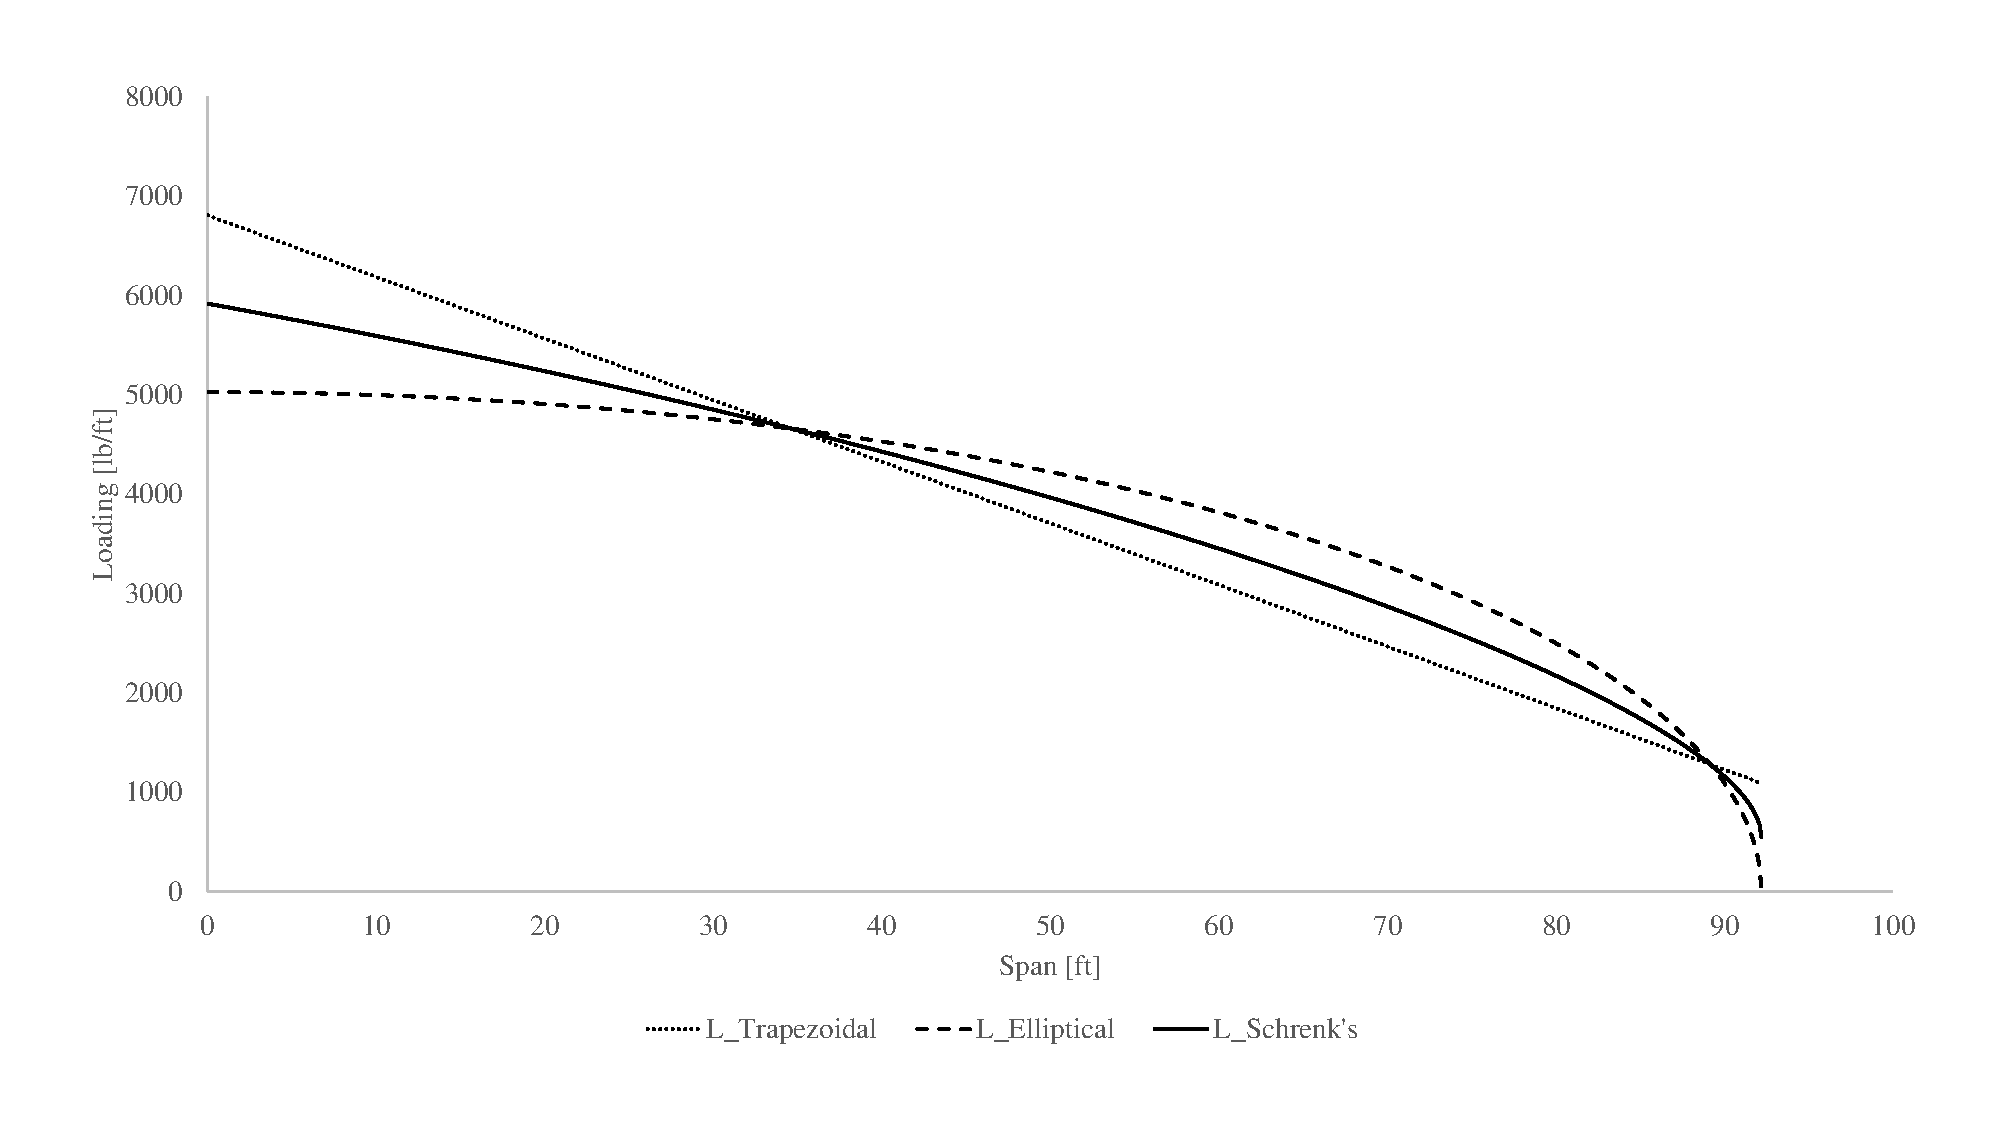
\includegraphics[width=1.0\linewidth]{Photos/Schrenks.pdf}
    \caption{Load Distribution Across the Half-span Wing}
    \label{schrenk}
\end{figure}

After estimating the load distribution on the wing, the internal forces of the wing are to be determined. Team Toucans implemented a numerical integration scheme, in which the Schrenk's diagram was integrated to obtain a shear diagram. This shear diagram was then integrated again to derive the bending moment diagram. The integration method of choice was the trapezoidal method. Both of these diagrams are modeled on the half-span of the wing, thereby assuming symmetry. Figures \ref{sheardiag} and \ref{momentdiag} show the Shear and Bending Moment diagrams as functions of half the span of the wing, respectively. Note that the shear loading and bending moments are zero at the tips and maximum at the center of the wing. 

\begin{figure}[H]
    \centering
    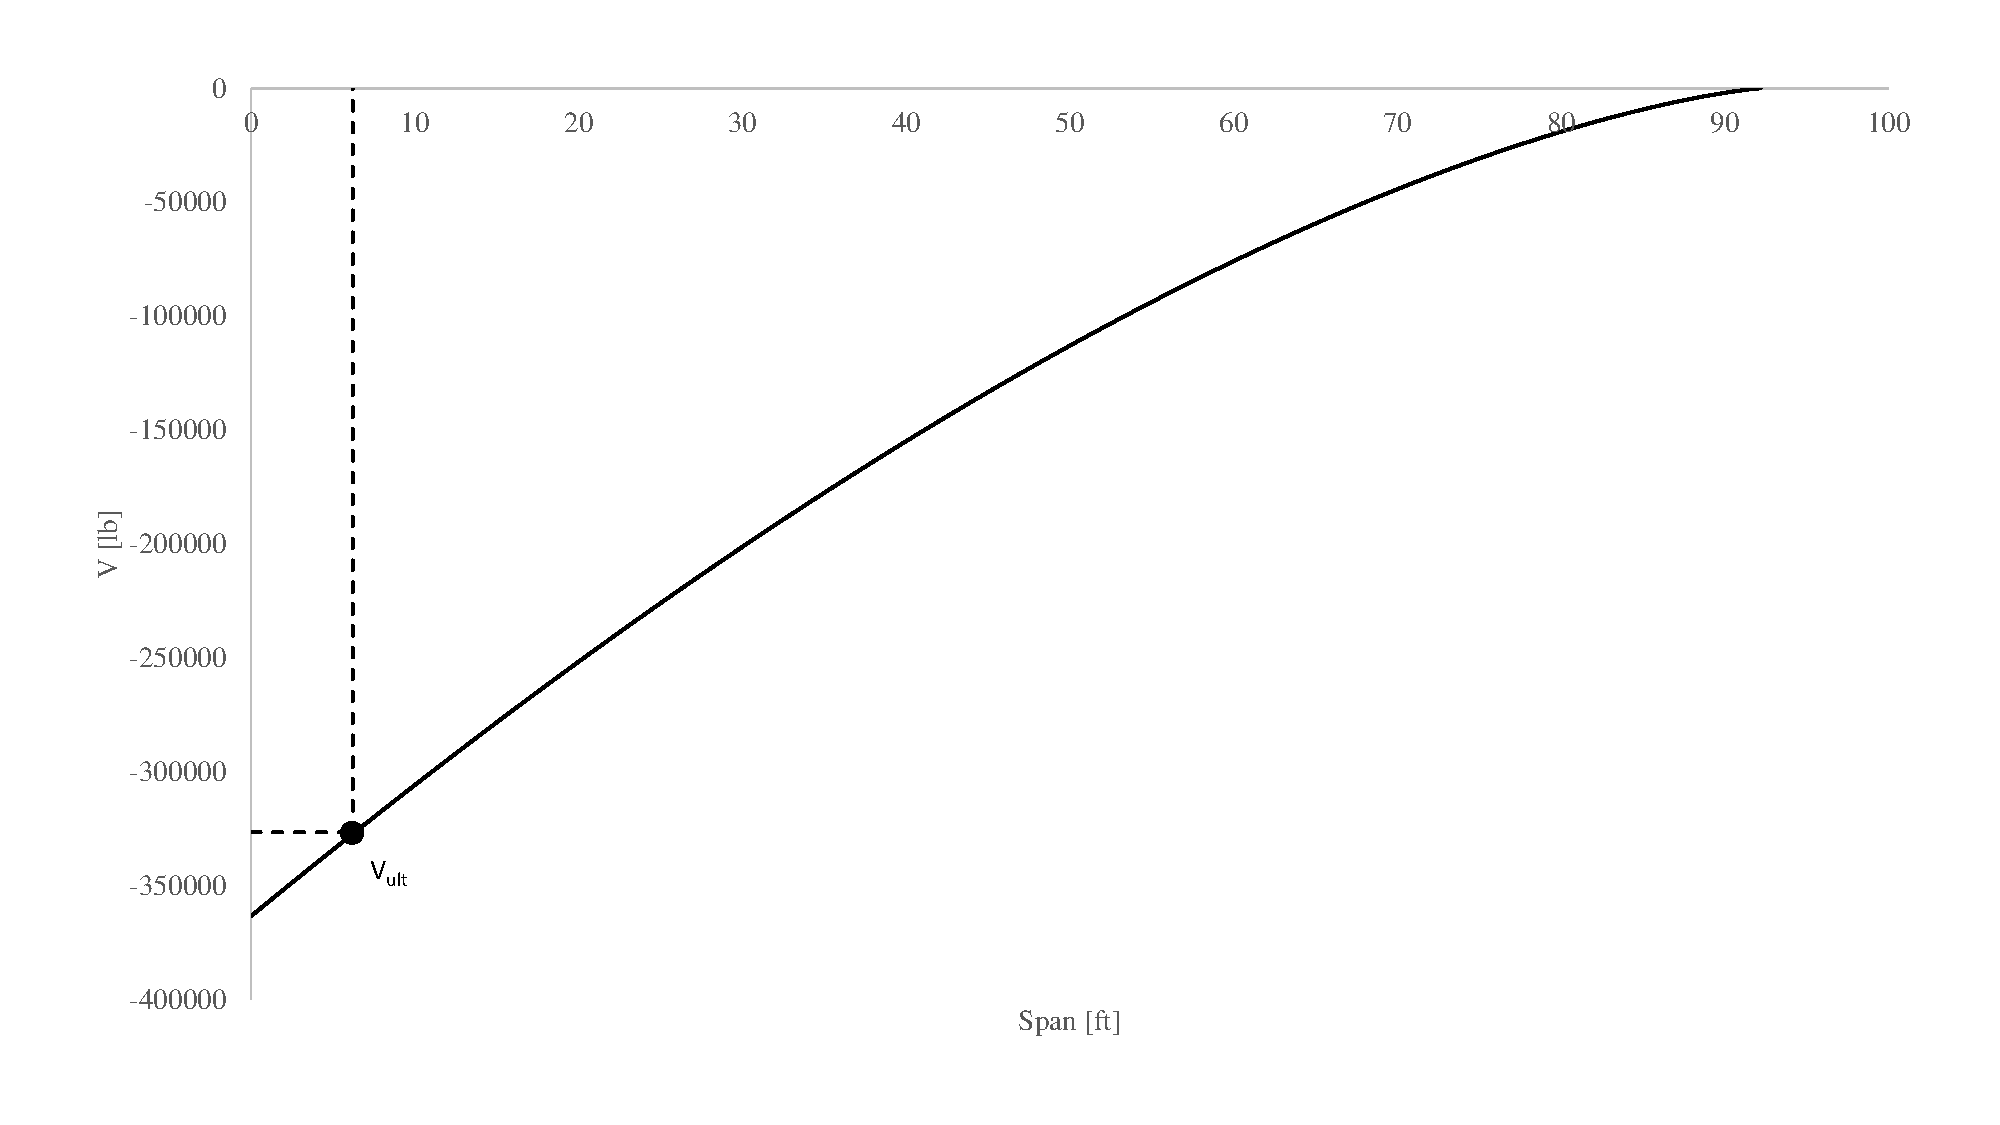
\includegraphics[width=1.0\linewidth]{Photos/Shear.pdf}
    \caption{Shear Diagram Across the Half-span Wing}
    \label{sheardiag}
\end{figure}

\begin{figure}[H]
    \centering
    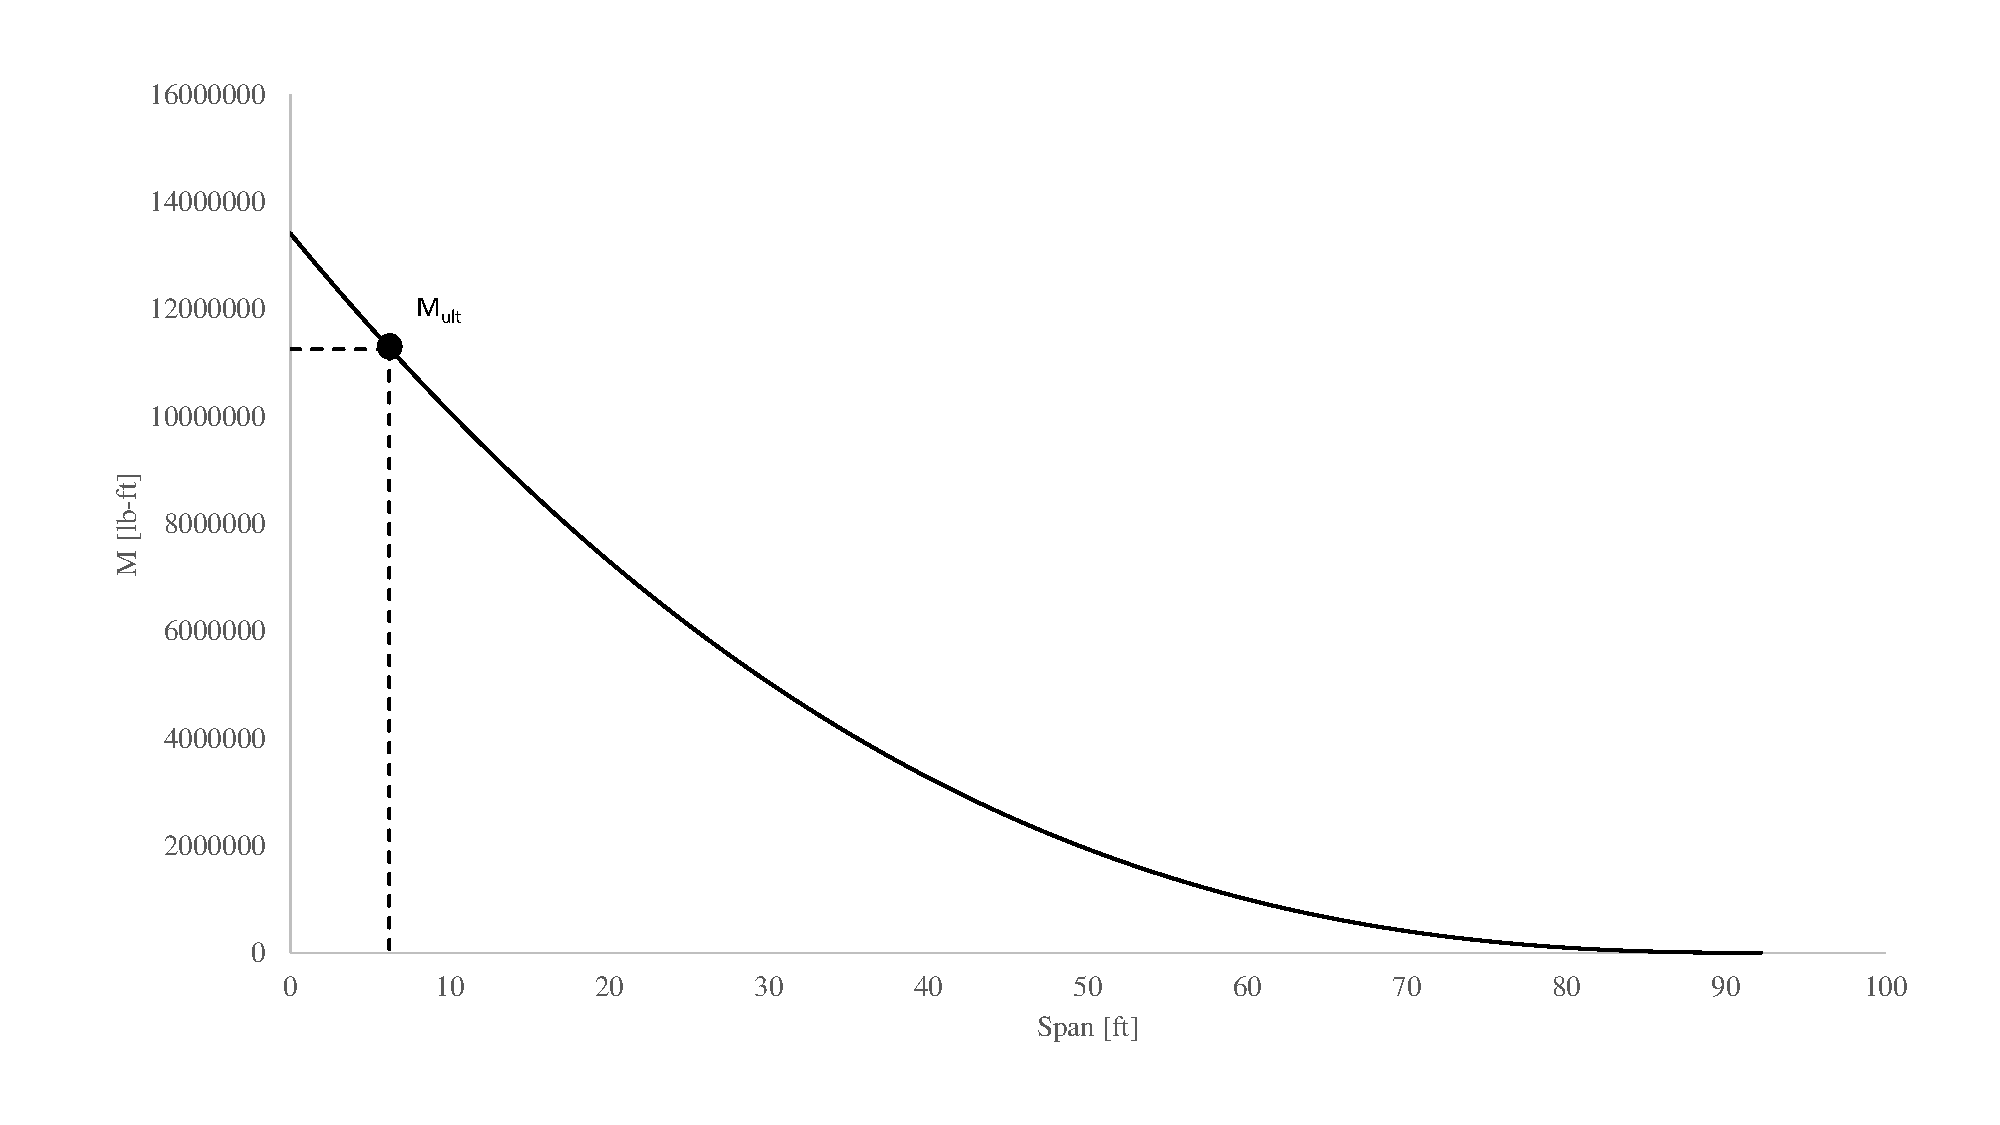
\includegraphics[width=1.0\linewidth]{Photos/Moment.pdf}
    \caption{Bending Moment Diagram Across the Half-span Wing}
    \label{momentdiag}
\end{figure}

\clearpage
Finally, the ultimate shear load and ultimate bending moment need to be determined. These can be estimated by estimating the distance from the center of the fuselage to the location of the wing attachment to the fuselage. This wing attachment location was estimated to be 6.2 ft from the center of the fuselage. This location is where the wing will feel the ultimate shear load and bending moment, which were estimated to be -327,000 lb and 11,276,000 lb-ft, respectively. These are represented in Figures \ref{sheardiag} and \ref{momentdiag} as black dots. 

\subsubsection{Load Paths}
As the wing is experiencing aerodynamic loads, those loads are transferred onto the structure of the aircraft. From the Schrenk's approximation of the lift distribution across the wing, the load then gets transferred onto the wing panels. From there, the loading transfers onto the spars, which lead to the wing box. Then, from the wing box, the loading goes into the fuselage, where the maximum loading occurs. The ribs on the wing absorb the shear produced by the bending moment from the lift distribution. Additionally, the engine also produces a load onto the wing. This loading follows a similar path, except it moves into the pylon first, then into the wing panels. From there, the load transfers into the spars, which moves into the wing box, and finally into the fuselage. Figure \ref{loadpath} shows a diagram of the load paths across half the aircraft, since it will be symmetric along the center line of the fuselage. 

\begin{figure}[H]
    \centering
    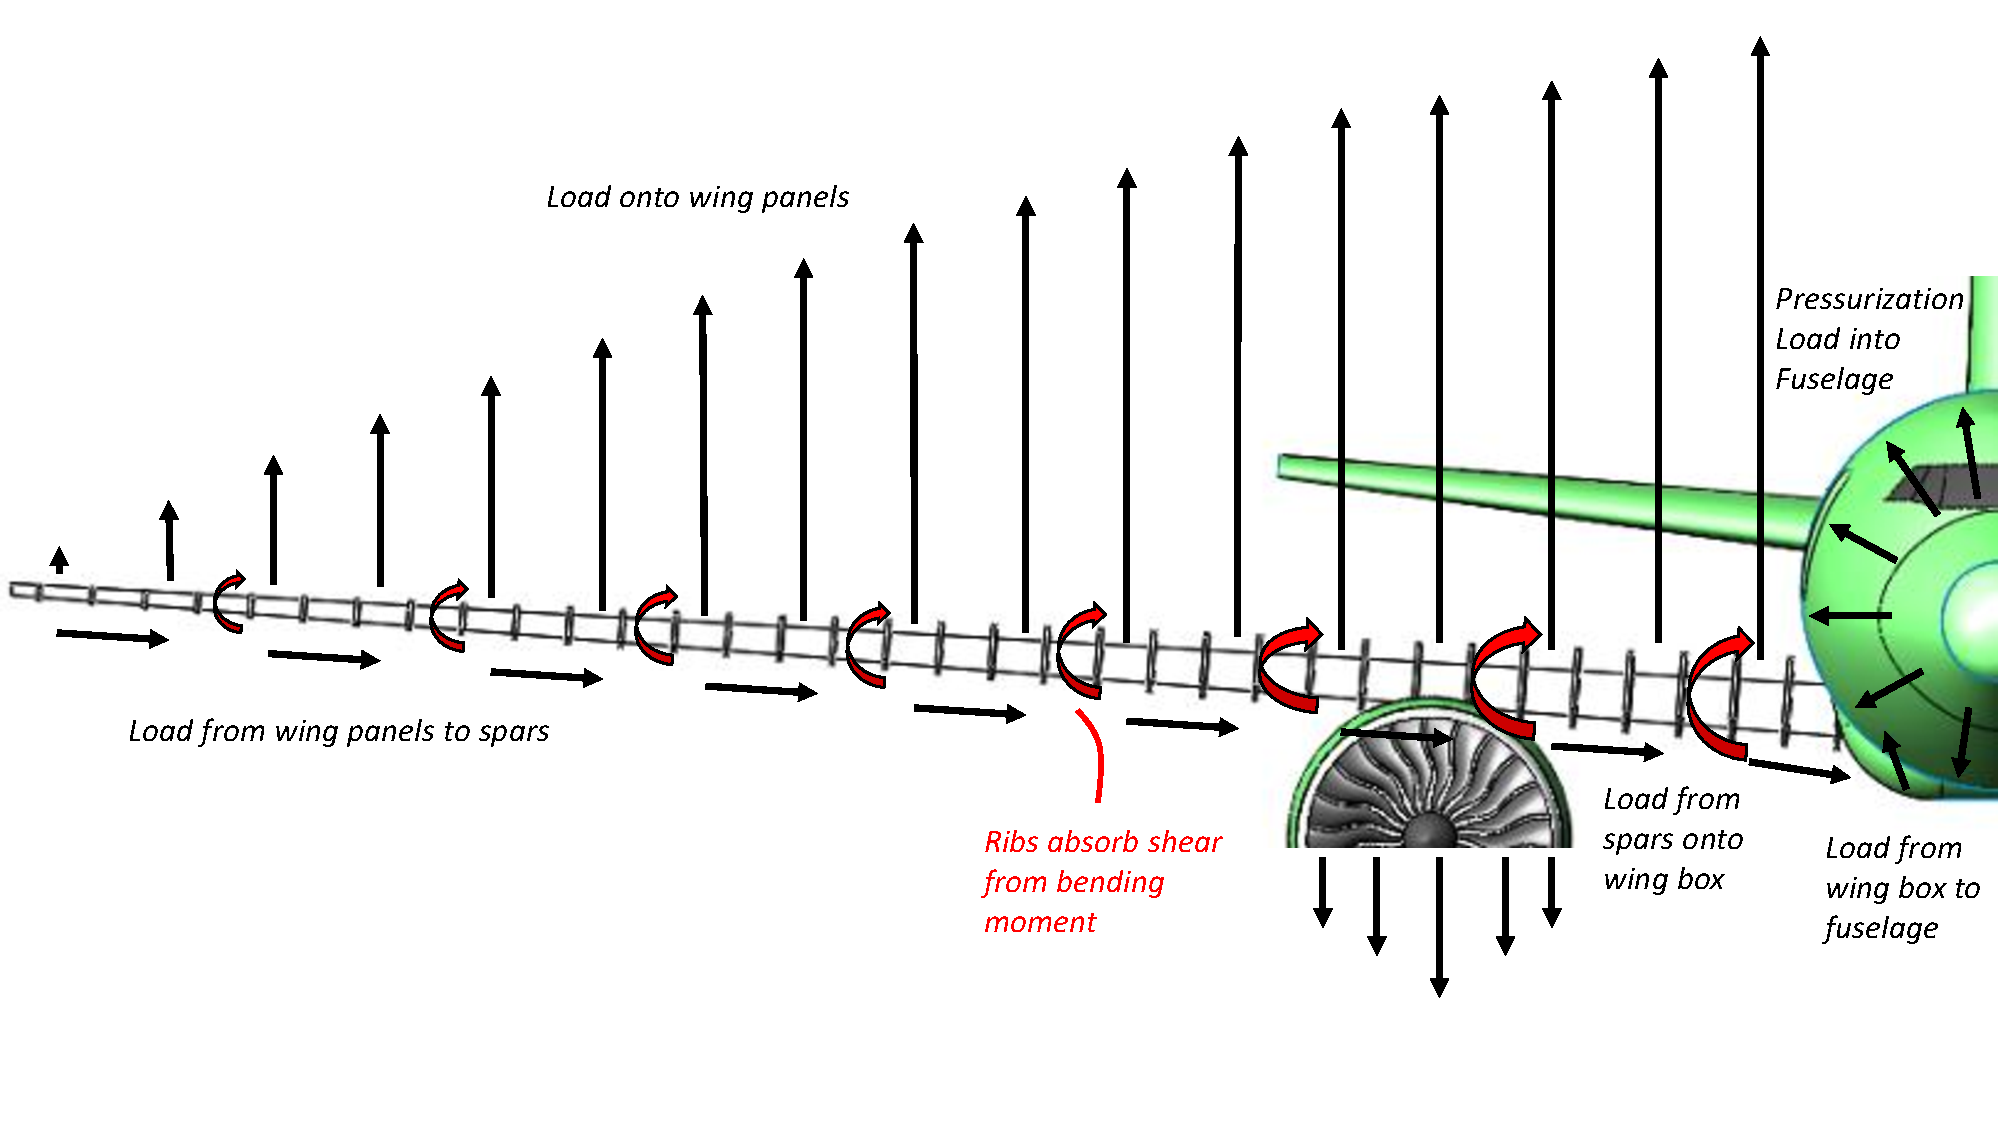
\includegraphics[width=1.0\linewidth]{Photos/Load_Path.pdf}
    \caption{Load Path of the Lift Distribution, Engine Weight, and Pressurization}
    \label{loadpath}
\end{figure}

\newpage
Furthermore, the aircraft will experience pressurization loads during cruise flight. According to the RFP \cite{RFP}, the aircraft will need to be pressurized to 8,000 ft pressure altitude above that altitude. Thus, there will be a pressure differential, specifically a max differential at the point where the aircraft is at its highest altitude. Since SAM Mk I will be starting at a cruise altitude of 37,000 and end at 41,000 ft, the last altitude height will carry the highest pressure differential in the aircraft. The fuselage will feel this differential as displayed in the load path diagram in Figure \ref{loadpath}.
Table \ref{tab:pres} displays the pressures the aircraft will be pressurized to, the pressure at 41,000 ft altitude, and the differential between both those values. 

\begin{table}[!h]
    \centering
    \caption{Pressure Differential}
    \begin{tabular}{|c|c|c|c|}\toprule 
     & \textbf{8,000 ft (Cabin)} & \textbf{41,000 ft} & \textbf{Difference} \\ \hline \hline
    \textbf{Pressure [psi]} & 10.92 & 2.59 & 8.32 \\ 
    \bottomrule
    \end{tabular}
    \label{tab:pres}
\end{table}

With this pressure difference comes a stress on the fuselage skin. This pressure differential results in a hoop stress that the fuselage feels. To calculate this stress, the hoop stress equation for a thin-walled pressure vessel was used, along with a skin thickness of 0.045 in. Table \ref{hoopstrs} displays the hoop stress felt by the fuselage.

\begin{table}[!h]
    \centering
    \caption{Hoop Stress of Fuselage}
    \begin{tabular}{|c|}\toprule 
    \textbf{Hoop Stress (8,000 ft) [psi]} \\ \hline
    26,200 \\ 
    \bottomrule
    \end{tabular}
    \label{hoopstrs}
\end{table}

\subsubsection{Load Cases of Interest}
\label{lcoi}
There are several cases of loads that apply to the aircraft, with some load cases being more significant than others. The highest loads experienced by the aircraft come from maneuver and gust loads, as described in the V-n diagram in Section \ref{subvn}. An example of a maneuvering load is turning, where the aircraft needs to be able to handle the amount of gs experienced when suddenly changing directions. The next important load case is during cruise flight. In particular, this segment of the mission experiences pressurization loads. This is significant because as altitude increases, the pressure outside the cabin will decrease while the inside cabin pressure stays at a constant value. This will create some bulging of the fuselage, which will put high stresses on the aircraft. Moreover, in cruise flight and climb and descent, the aircraft will experience aerodynamic loads, as described in Section \ref{winlod}. This will put stresses across the span of the wing, which will lead to high stress at the interface of the wing and fuselage. Another load case of interest corresponds to the aircraft landing. This puts stresses not only on the landing gears, but this transfers to the fuselage and wing of the aircraft. Finally, the taxi segment of the mission profile experiences stresses on the aircraft. While the aircraft is not actually flying at this stage, it still experiences loads due to any turns or bumps it passes. While these are not as significant as maneuvering and gust loads, these loads are still an important aspect to take into consideration when analyzing the loads experienced by the aircraft.



% \textcolor{red}{
% \begin{itemize}
%     \item Discuss any analysis supporting the sizing analysis.
%     \item Discuss future work.
%     \item AIAA: A V -n diagram for the aircraft with identification of necessary aircraft velocities and design load factors.
%     Required gust loads are specified in 14 Code of Federal Regulations (CFR) Part 25
%     \item AIAA: Materials selection for main structural groups and general structural design, including layout of primary airframe structure as well as the strength capability of the structure
%     and how that compares to what is required at the ultimate load limits of the aircraft.  The maximum dive speed shall be specified.
% \end{itemize}}

\subsection{Wing Structure Analysis (\textit{CE})}
In order to determine if the wing structure can withstand the loads on the wings during a typical flight mission, a computer simulation using SolidWorks was completed. The wing structure seen in Fig. \ref{fig:wing_structure} was loaded along each spar with a percentage of the Schrenk's loading approximation defined in Section \ref{winlod}. It was estimated that the front spar carries 85\% of the load, and the rear spar carries 15\% of the load due to their location relative to the lifting line at the quarter chord. The wing structure was modelled with the Hexcel CFRP material defined in \ref{tab:material_properties}. The wingbox was assumed to be a solid fixture, such that it behaves like a strongback. In Figs. \ref{fig:wing_displacement} and \ref{fig:wing_stress}, the FEA results of the model can be seen.

\begin{figure}[!h]
    \centering
    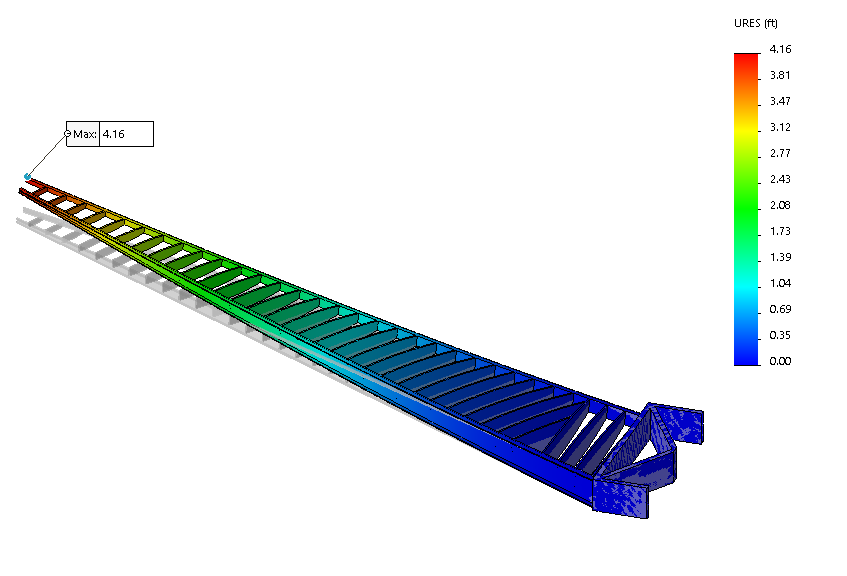
\includegraphics[width=\linewidth]{Photos/structuresandloads/Wing Displacement Composite.PNG}
    \caption{SAM Mk I Composite Wing Displacement}
    \label{fig:wing_displacement}
\end{figure}
\begin{figure}[!h]
    \centering
    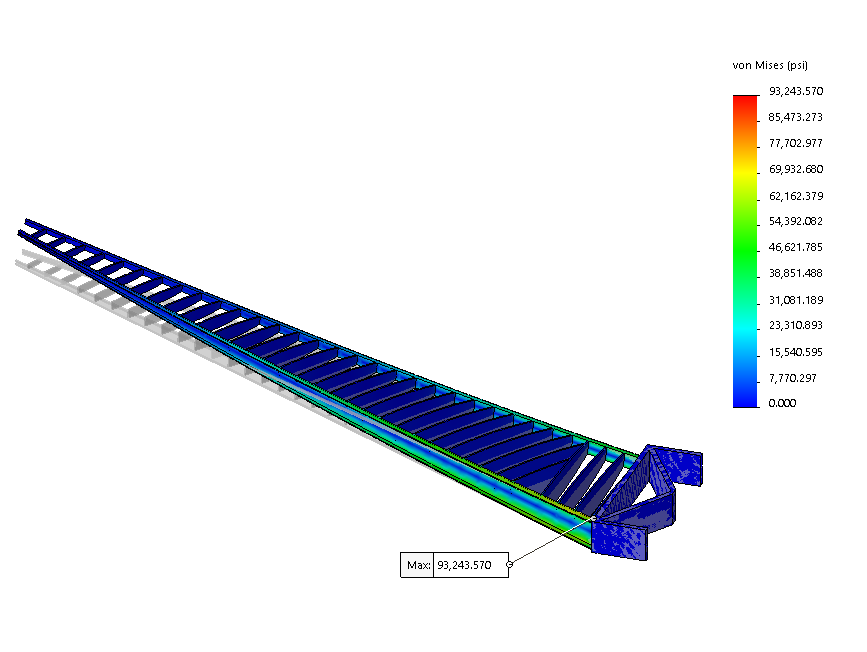
\includegraphics[width=\linewidth]{Photos/structuresandloads/Wing Stress Composite.PNG}
    \caption{SAM Mk I Composite Wing Stress}
    \label{fig:wing_stress}
\end{figure}
\FloatBarrier

From the simulation, it was found that the displacement at the tip of the wing was 4.16 feet, and the maximum stress was 93.2 ksi at the junction of the wing and wingbox. This maximum stress is well within the ultimate tensile strength of the composite material defined in Table \ref{tab:material_properties}. 

As a trade study, the same wing geometry was simulated using the 2024-T4 aluminum defined in Table \ref{tab:material_properties}. This simulation is not idealized, as the wing geometry is designed for composite manufacturing. Regardless, the results of the simulation can be seen in Figs. \ref{fig:wing_displacement_al} and \ref{fig:wing_stress_al}.

\begin{figure}[!h]
    \centering
    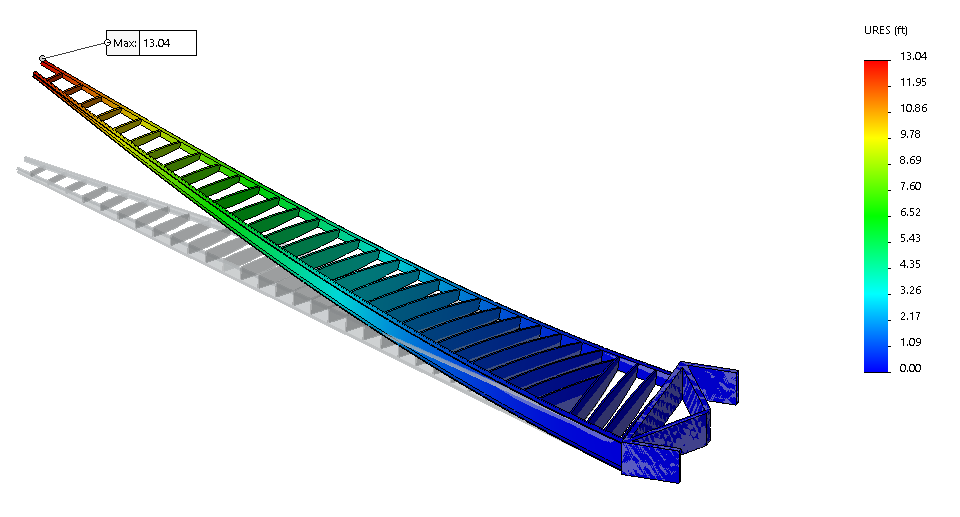
\includegraphics[width=\linewidth]{Photos/structuresandloads/Wing Displacement Aluminum.PNG}
    \caption{SAM Mk I Aluminum Wing Displacement}
    \label{fig:wing_displacement_al}
\end{figure}
\begin{figure}[!h]
    \centering
    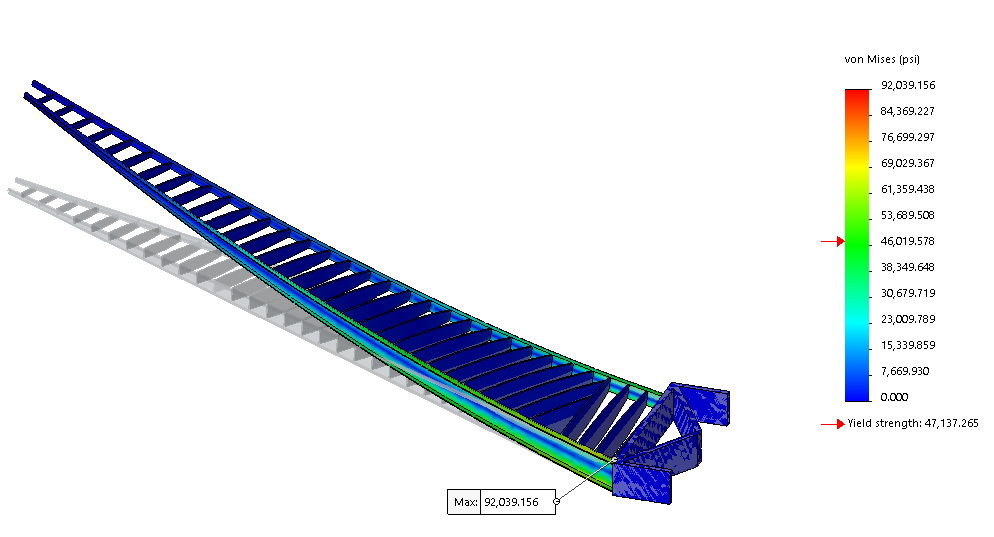
\includegraphics[width=\linewidth]{Photos/structuresandloads/Wing Stress Aluminum.PNG}
    \caption{SAM Mk I Aluminum Wing Stress}
    \label{fig:wing_stress_al}
\end{figure}
\FloatBarrier


\clearpage
It can be seen that the displacement at the tip of the wing under the same loading described previously is 13.04 feet, and the maximum stress at the root if the wing is again 92.0 ksi. This stress is higher than the yield stress of the 2024-T4 aluminum alloy, meaning the geometry fails under loading. This issue can be mitigated by increasing the cross sectional area of the wing spars by increasing the leg and web thicknesses. 

\FloatBarrier
\subsection{Landing Gear (\textbf{CE})}
\label{section: Landing Gear}
\subsubsection{Configuration}
The aircraft will feature three sets of retractable landing gear customary of that found on similar aircraft within the aircraft featured in the trade study found in Table \ref{tab:trade_params}. The nose gear will be composed of two wheels, and the main gear will consist of two symmetric sets of six wheels each, three wheels in a line on each side of each set. All of the gear will be hydraulically mounted to dampen the impact seen upon touchdown, as well as hydraulically actuated. The "tricycle" arrangement is traditionally seen due to both the stability on uneven surfaces as well as the weight distribution of the aircraft.  The front gear will also feature the main taxi light. Landing gear doors will be utilized in order to increase performance characteristics by reducing drag. 

Given the main configuration stated above, the landing gear was sized such that the main struts and nose struts were able to carry the maximum dynamic and static loads, defined in Raymer. \cite{raymer} The primary Oleo cylinder for the main landing gear is sized to be 16 inches in diameter, whereas the front Oleo strut cylinder is sized to be 10 inches in diameter. The height and longitudinal placement of the landing gear was primarily sized given the clearance angle of approximately 12 degrees, seen in Fig. \ref{fig:gear_angle}, at take off and the maximum static and dynamic loads seen by each gear. \cite{raymer} In Fig. \ref{fig:landing_gear_CG}, it can be seen that main landing gear is placed aft of the MTOW CG limit, labelled as "AFT" in the figure. Given this, it can be assumed that the aircraft will be stable on the ground at MTOW.

\begin{figure}[!h]
    \centering
    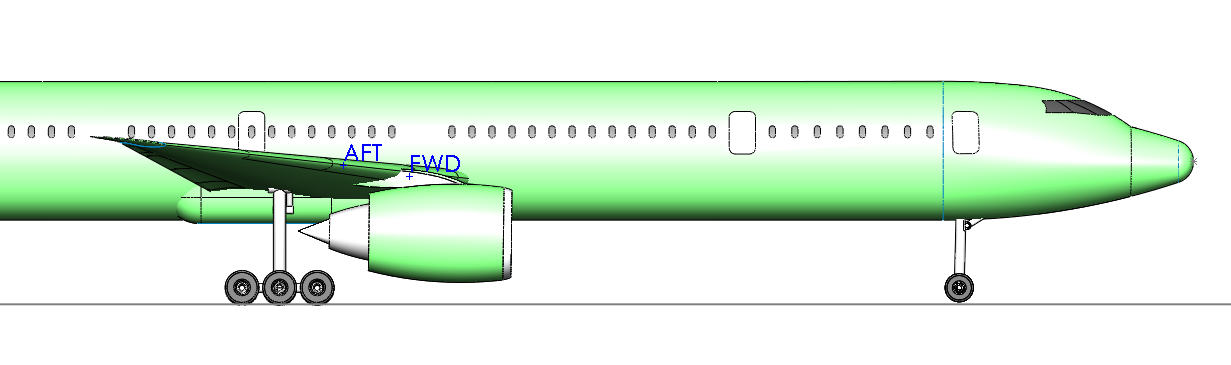
\includegraphics[width=\linewidth]{Photos/landinggear/LG Close Side View with CG.PNG}
    \caption{SAM Mk I Landing Gear in Relation to CG Limits}
    \label{fig:landing_gear_CG}
\end{figure}
\begin{figure}[!h]
    \centering
    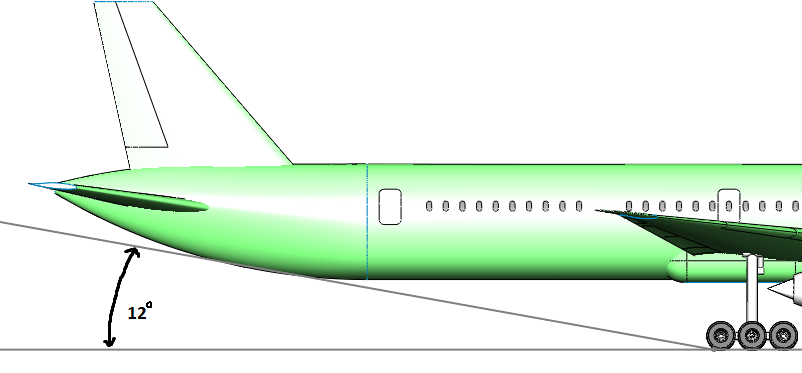
\includegraphics[width=\linewidth]{Photos/landinggear/Landing Gear Angle.PNG}
    \caption{SAM Mk I Landing Gear Maximum Takeoff Angle}
    \label{fig:gear_angle}
\end{figure}
\FloatBarrier
The main and nose landing gear bogeys can be seen in Figs. \ref{fig:main_gear} and \ref{fig:nose_gear} respectively. 

\begin{figure}[!h]
  \centering
  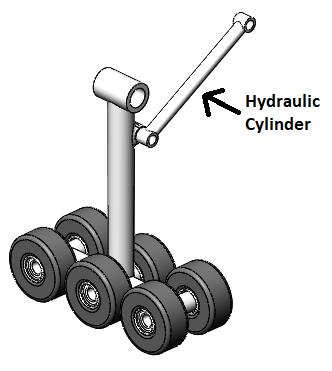
\includegraphics[width=.5\linewidth]{Photos/landinggear/Main Gear ISO.PNG}
  \captionof{figure}{Main Gear Bogey}
  \label{fig:main_gear}
\end{figure}
\begin{figure}[!h]
  \centering
  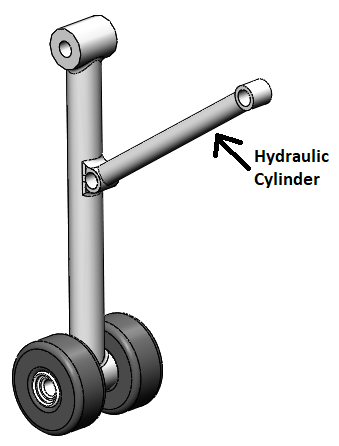
\includegraphics[width=.4\linewidth]{Photos/landinggear/Nose Gear ISO.PNG}
  \captionof{figure}{Nose Gear Bogey}
  \label{fig:nose_gear}
\end{figure}
\FloatBarrier

\subsubsection{Kinematics}
The landing gear is designed in such a way which allows seamless stowage into the belly of the aircraft. In Figs. \ref{fig:main_landing_kin} and \ref{fig:nose_landing_kin}, the kinematics of the main and nose landing gear are shown. As seen, both the main and nose landing gear stow into the aircraft without interference. The main landing gear stow behind the wingbox to eliminate interference issues.

\begin{figure}[!h]
    \centering
    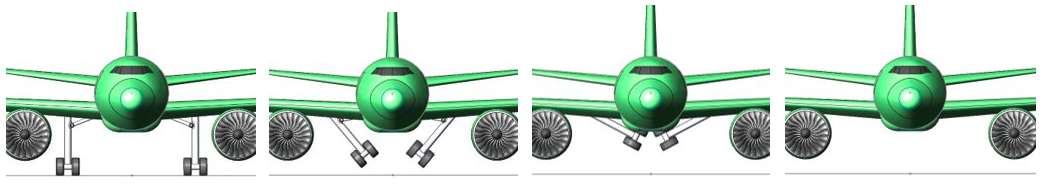
\includegraphics[width=\linewidth]{Photos/landinggear/Main Gear Kinematics.PNG}
    \caption{SAM Mk I Main Landing Gear Kinematics}
    \label{fig:main_landing_kin}
\end{figure}

\begin{figure}[!h]
    \centering
    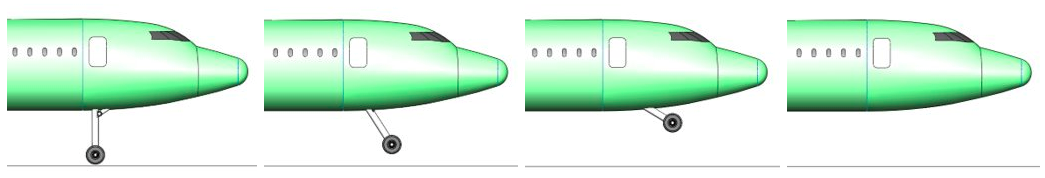
\includegraphics[width=\linewidth]{Photos/landinggear/Nose Gear Kinematics.PNG}
    \caption{SAM Mk I Nose Landing Gear Kinematics}
    \label{fig:nose_landing_kin}
\end{figure}

\subsubsection{Tire Selection (JJ)}
With the SAM Mk I falling within the weight and size boundaries of established commercial aircraft, designing to utilize tires already available from known manufacturers saves cost and time, and also mitigates the threat of setbacks due to developmental overruns from the manufacturer. Bridgestone was selected as a launch supplier for both the nose (two) and main (twelve) tires using existing tires from their APR line first introduced for the Boeing 777-300ER/200LR in 2004 \cite{bridgestonetire}.  Their listed specifications, as published by Bridgestone \cite{bridgestonetire}, are below in Table \ref{tab:tires}.  Per FAA FAR Part §25.733 \cite{cfr}, the tires will be filled with dry nitrogen to mitigate issues caused by dioxygen, a powerful oxidizer, at high heats as well as moisture, both found in ambient air. 

\begin{table}[!h]
    \centering
        \caption{Tire Specifications}
    \begin{tabular}{|c||c|c|>{\centering}p{.8in}|>{\centering}p{.7in}|>{\centering}p{.95in}|c|}\toprule
         & \textbf{Size} & \textbf{Ply Rating} & \textbf{Speed Rating [MPH]} & \textbf{Rated Load [lb]} & \textbf{Average Weight [lb]} & \textbf{Model} \\\hline \hline
         \textbf{Main} & 52x21.0R22 & 36 & 235 & 66,500 & 266 & APR07700 \\ \hline
         \textbf{Nose} & 43x17.5R17 & 32 & 235 & 44,500 & 156 & APR06600 \\ \hline
    \end{tabular}
    \label{tab:tires}
\end{table}

\clearpage
% \textcolor{red}{
% \begin{itemize}
%     \item Discuss landing gear sizing, tire sizing, loads, and retraction system.
%     \item Include CAD drawings with landing gear extended and stowed.
%     \item Discuss pressurization (if used).
%     \item Consider merging into Structures as a sub section
% \end{itemize}}